\section{Генетическое программирование.}
Идея состоит в выращивании программ (не код на питоне а что то более абстрактное) путем эволюции
Для описания можно использовать:
\begin{itemize}
\item Символьная регрессия
\item Конечные автоматы-распознаватели
\end{itemize}
Также мы можем представлять программы в виде деревьев:
Особи=решения: деревья разбора программ. Приспособленность: основана на запуске закодированной программы. 
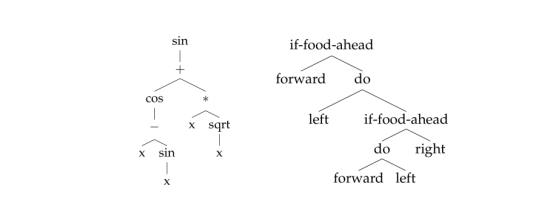
\includegraphics{images/evolv_gen}
Дерево состоит из следующих компонентов: Функции нулевой арности (листья) и Функции ненулевой арности (внутренние вершины).
Функции нулевой арности могут быть:
\begin{itemize}
	\item Константы
	\item Переменные
	\item Эфемерные константы: генерируются в момент первого обращения
	\item Параметры: можно дополнительно настраивать при вычислении приспособленности
	\item Вызовы других деревьев (функции)
\end{itemize}
Функции ненулевой арности (внутренние вершины) могут быть:
\begin{itemize}
	\item Арифметические и логические операции
	\item Управляющие операторы (if-then-else, while и тд )
	\item Произвольные функции
\end{itemize}
Узлы дерева также могут иметь тип что также надо учитывать. 
Инициализация дерева:
\begin{enumerate} 
	\item Необходимо ставить ограничения на глубину решения 
	\item Grow: глубина каждого листа не превышает максимальную
	\item F ull: глубина каждого листа равна максимальной
	\item Ram pedHal fAndHal f: с вероятностью p = 0.5 вызываем в поддереве Grow, иначе Full
	\item Можем балансировать между максимальной глубиной листа
\end{enumerate} 
Мутации:
\begin{itemize}
Заменить поддерево случайно сгенерированным деревом
	\item Заменить внутреннюю вершину одним из ее детей
	\item Заменить операцию во внутренней вершине случайной операцией той же арности
	\item Поменять детей внутренней вершины, если в этом есть смысл
	\item Поменять два случайно выбранных поддерева
	\item Мутировать константу в листе
	\item чето еще
\end{itemize}
Кроссовер:
\begin{itemize}
	\item Как правило, обмен поддеревьями
	\item Часто встречающаяся рекомендация: с p = 0.1 выбирать для обмена лист, иначе внутреннюю вершину
	\item Может радикально изменить фенотип, но при обмене похожими поддеревьями «можно жить»
\end{itemize}
Можем генерировать программы используя стековые языки (примитивные инструкции). 
Соотвественно тогда для решения нам не нужны деревья а просто список инструкций переменной длины. 
В случае с достаточно мощными языками программы могут генерировать и запускать код, заниматься самомодификацией
